\documentclass[12pt,a4paper]{article}
\usepackage{graphicx}
\usepackage[utf8]{inputenc}
\usepackage{titling}
\usepackage{hyperref}
\usepackage{fancyhdr}
\usepackage[headsep=1.5cm]{geometry}
\usepackage{float} % Para que los floats se estén quietecitos

%%% LISTINGS %%%
\usepackage{listings}
\usepackage{lstautogobble}  % Fix relative indenting
\usepackage{color}          % Code coloring
\usepackage{zi4}            % Nice font

\definecolor{bluekeywords}{rgb}{0.13, 0.13, 1}
\definecolor{greencomments}{rgb}{0, 0.5, 0}
\definecolor{redstrings}{rgb}{0.9, 0, 0}
\definecolor{graynumbers}{rgb}{0.5, 0.5, 0.5}

\usepackage{listings}
\lstset{
    autogobble,
    columns=fullflexible,
    showspaces=false,
    showtabs=false,
    breaklines=true,
    showstringspaces=false,
    breakatwhitespace=true,
    escapeinside={(*@}{@*)},
    commentstyle=\color{greencomments},
    keywordstyle=\color{bluekeywords},
    stringstyle=\color{redstrings},
    numberstyle=\color{graynumbers},
    basicstyle=\footnotesize\ttfamily,
    frame=l,
    framesep=12pt,
    xleftmargin=12pt,
    tabsize=4,
    captionpos=b
}
%%% /LISTINGS %%%





\title{Configuració de Ports}
\author{
    Iván Canales% Martín
    \\
    Xavier Ripoll% Echeveste
}

\date{9 de març de 2018}

\pagestyle{fancy}
\fancyhf{}

% Head
\lhead{\small\theauthor}
\chead{\small Programació d'Arquitectures\\Encastades}
\rhead{\small Pràctica 2:\\Configuració de Ports}

% Foot
\cfoot{\thepage}

\begin{document}

%%%%%%%%%%%%%%%%%%%%%%%%%%%%%%%%%%%%
%%%%%%%%%%%% TITLE PAGE %%%%%%%%%%%%
%%%%%%%%%%%%%%%%%%%%%%%%%%%%%%%%%%%%

% un dia de estos lo hago plantilla
\begin{titlepage}
	\centering
	{\scshape\LARGE Universitat de Barcelona \par}
	\vspace{2cm}
	{\scshape\Large Pràctica 2:\par}
	\vspace{1cm}
	{\huge\bfseries \thetitle \par}

    \vfill
    \large\theauthor
	\vfill
	\raggedleft

    \par

    %\hrulefill\par
    {\scshape Programació d'Arquitectures Encastades\par}
    \texttt{}{Curs 2017-2018\par} %Universitat de Barcelona
    \thedate

% Bottom of the page

\end{titlepage} \pagebreak
%%%%%%%%%%%%%%%%%%%%%%%%%%%%%%%%%%%%%%%%
\section{Introducció}

\subsection{Objectius}
% Què es vol fer a la pràctica.

En la pràctica es pretén introduir els GPIOs (\textit{General Purpose
Input/Output} o entrades i sortides de propòsit general). Per fer-ho,
programarem algunes entrades del robot (el \textit{joystick} i dos botons) per
a que modifiquin algunes sortides (la pantalla de la placa superior i uns LEDs),
segons la següent taula:

\begin{table}[H]
  \centering
  \begin{tabular}{|l||l|l|l||l|} \hline
    Estat & LED B    & LED G    & LED R    & Botó   \\ \hline
    1     & 1        & 1        & 1        & S1     \\ \hline
    2     & 0        & 0        & 0        & S2     \\ \hline
    3     & 1        & 1        & 1        & Left   \\ \hline
    4     & 0        & 1        & 1        & Right  \\ \hline
    5     & 1        & 0        & 1        & Up     \\ \hline
    6     & 1        & 1        & 0        & Down   \\ \hline
    7     & Invertir & Invertir & Invertir & Center \\ \hline
  \end{tabular}
\end{table}

A més a més, els controls horitzontals del \textit{joystick} marquen la direcció
en què circula un senyal a través dels LEDs de la placa inferior, i els controls
verticals, la velocitat a la que es mou el senyal.

Per a que aquests dos comportaments es realitzin correctament i en temps real,
cal que considerem la \textit{sincronia} del codi. Per això emprem uns mètodes
anomenats \textit{handlers} que són cridats quan hi ha una interrupció (en el
nostre cas, quan es prem un botó o el \textit{joystick}), i és important que
qualsevol tasca que realitzem en el bucle principal no sigui bloquejant.

\subsection{Recursos utilitzats}
% Quins recursos del Microcontrolador, Placa d’Experimentació i Robot es fan servir.
De la placa \textit{Boosterpack MK II} volem fer servir:

\begin{itemize}
    \item Entrades: el \textit{joystick}, els polsadors S1 i S2
    \item Sortides: el LED RGB
\end{itemize}

De la Placa d'experimentació, farem servir els vuit LEDs del port P7.

De la placa d'interfície farem servir els 8 LEDs del port 8 (com sortida).

\subsection{Configuració dels recursos}
% Com s’han configurat els diferents recursos.
\subsubsection{Configuració dels LEDs}
Es posen els LEDs RGB (pins P2.6, P2.4 i P5.6 respectivament) com a sortides ($DIR = 1$) digitals ($SEL0 = SEL1 = 0$) i es posen a 0 (apagats).

\begin{lstlisting}[language=C]
P2DIR |=  0x50; //Pines P2.4 (G), 2.6 (R) como salidas Led (RGB)
P5DIR |=  0x40; //Pin P5.6 (B)como salida Led (RGB)
P2OUT &= ~0x50; //Inicializamos Led RGB a 0 (apagados)
P5OUT &= ~0x40; //Inicializamos Led RGB a 0 (apagados)
\end{lstlisting}

\subsubsection{Configuració dels botons}

Es posen els botons com entrades ($DIR = 0$) digitals ($SEL0 = SEL1 = 0$). Volem que la transició sigui en el flanc de pujada ($IES = 0$). finalment activem les interrupcions i netegem els flags.

\begin{lstlisting}[language=C]
//Boton S1
P5DIR  &= ~0x02; //Pin P5.1 como entrada
P5SEL0 &= ~0x02; //Pin P5.1 como I/O digital,
P5SEL1 &= ~0x02; //Pin P5.1 como I/O digital,
P5IES  &= ~0x02; // con transicion L->H
P5IE   |=  0x02; //Interrupciones activadas en P5.1,
P5IFG   =     0; //Limpiamos todos los flags
\end{lstlisting}

\begin{lstlisting}[language=C]
//Boton S2 del MK II:
P3DIR  &= ~0x20; //Pin P3.5 como entrada
P3SEL0 &= ~0x20; //Pin P3.5 como I/O digital,
P3SEL1 &= ~0x20; //Pin P3.5 como I/O digital,
P3IES  &= ~0x20; // con transicion L->H
P3IE   |=  0x20; //Interrupciones activadas en P3.5
P3IFG   =     0; //Limpiamos todos los flags de las interrupciones del puerto 3
\end{lstlisting}

\subsubsection{Configuració del joystick}

De la mateixa manera que els botons, es posen els bits del \textit{joystick} com entrades ($DIR = 0$) digitals ($SEL0 = SEL1 = 0$) amb transició per flanc de pujada.
\begin{lstlisting}[language=C]
//PIN 4
P4DIR  &= ~(BIT1 + BIT5 + BIT7); //Posar com entrades,
P4SEL0 &= ~(BIT1 + BIT5 + BIT7); //Posar a I/O digital,
P4SEL1 &= ~(BIT1 + BIT5 + BIT7); //
P4REN  |=   BIT1 + BIT5 + BIT7;  //Activar resistencia pullup
P4OUT  |=   BIT1 + BIT5 + BIT7;  //
P4IE   |=   BIT1 + BIT5 + BIT7;  //Interrupcions activadas
P4IES  &= ~(BIT1 + BIT5 + BIT7); //Interrupcions L->H
P4IFG   = 0;    //Netejar flags

//PIN 5
P5DIR  &= ~(BIT4 + BIT5); //Posar com entrades,
P5SEL0 &= ~(BIT4 + BIT5); //Posar a I/O digital,
P5SEL1 &= ~(BIT4 + BIT5); //
P5REN  |=   BIT4 + BIT5 ; //Activar resistencia pullup
P5OUT  |=   BIT4 + BIT5 ; //
P5IE   |=   BIT4 + BIT5 ; //Activar intrrupcions
P5IES  &= ~(BIT4 + BIT5); //Interrupcions L->HL->H
P5IFG = 0;    //Netejar flags
\end{lstlisting}

\subsubsection{Configuració dels LEDs del port P7}

Cal que posem tots els LEDs como a salida digital (igual que els LEDs RGB).

\begin{lstlisting}[language=C]
P7DIR  |= 0xFF; // Todos de salida
P7SEL0 &= 0x00; // Todos GPIO
P7SEL1 &= 0x00;
P7OUT  &= 0x00;  // Todos apagados
\end{lstlisting}

%\subsection{Funcions utilitzades}
% Com i per quines funcions es fan servir.


\subsection{Problemes}
% Problemes que han sorgit (que no siguin de compilació) i com s’han solucionat.
Durant la implementació de la practica vam descartar l'ús de \texttt{delay\_t} y en la gestió del moviment dels leds del port P7, doncs és una funció bloquejant, i volem que encara que els leds es moguin es pugin modificar els estats.

En quant a hardware, vam trobar que un dels leds del port P7 no funcionaba, fet que va dificultar el testeig del programa.

\subsection{Conclusions}

\section{Comentari del codi}


\subsection{do...while}

\begin{lstlisting}[language=C]
void delay_t(uint32_t temps)
{
    volatile uint32_t i = temps;
    do
    {
        i--;
    }
    while (i > 0); // decrementem mentres que i sigui > 0: fem i passos
}
\end{lstlisting}

\subsection{switch...case}

Cal notar que per qüestions de legibilitat hem suprimit els comentaris que detallen la taula d'estats

\begin{lstlisting}[language=C]
void PORT3_IRQHandler(void)
{   //interrupcion del pulsador S2
    uint8_t flag = P3IV; //guardamos el vector de interrupciones. De paso, al acceder a este vector, se limpia automaticamente.
    P3IE &= 0xDF;  //interrupciones del boton S2 en port 3 desactivadas
    estado_anterior = 0; // activa el cambio de estado

    switch (flag)
    {
    // 0x0C == BIT5
    case 0x0C: // P3.5
        // si el bit activat es el 5 es el pulsador S2
        estado = 2;
        break;
    }

    P3IE |= BIT5;   //interrupciones S2 en port 3 reactivadas
}
\end{lstlisting}
\textit{Nota: El bloc switch no és necessari però es posa per raons d'extensibilitat}

\begin{lstlisting}[language=C]
void PORT4_IRQHandler(void)
{
    uint8_t flag = P4IV; //guardamos el vector de interrupciones. De paso, al acceder a este vector, se limpia automaticamente.
    P4IE &= 0x5D;   //interrupciones Joystick en port 4 desactivadas
    estado_anterior = 0; // activa el cambio de estado

    switch (flag)
    {
    case 0x0C: // P4.5
        // se activa joystick derecha
        estado = 4;
        break;
    case 0x10: // P4.7
        // se activa joystick izquierda
        estado = 3;
        break;
    case 0x04: // P4.1
        // se activa joystick medio
        estado = 7;
        break;
    }

    P4IE |= 0xA2;   //interrupciones Joystick en port 4 reactivadas
}
\end{lstlisting}

\begin{lstlisting}[language=C]
//ISR para las interrupciones del puerto 5:
void PORT5_IRQHandler(void)
{
    uint8_t flag = P5IV; //guardamos el vector de interrupciones. De paso, al acceder a este vector, se limpia automaticamente.
    P5IE &= 0xCD;   //interrupciones Joystick y S1 en port 5 desactivadas
    estado_anterior = 0; // activa el cambio de estado


    switch (flag)
    {
    case 0x0A: // P5.4
        // activado joystick arriba
        estado = 5;
        break;
    case 0x0C: // P5.5
        // activado joystick abajo
        estado = 6;
        break;
    case 0x04: // P5.1
        // activado S1
        estado = 1;
        break;
    }

    P5IE |= 0x32;   //interrupciones Joystick y S1 en port 5 reactivadas
}
\end{lstlisting}

\subsection{if i for}

En la funció \texttt{main} farem el handle de les subrutines. Notem que fem que els bits del port P7 no aturin el bucle quan es delspacen.

\begin{lstlisting}[language=C]
void main(void)
{
    // Declaracion de variables
    uint32_t retraso_leds;
    uint32_t time_elapsed;
    uint8_t  izquierdaderecha;
    uint8_t  temp;
    uint8_t  led_actual;

    WDTCTL = WDTPW + WDTHOLD; // Paramos el watchdog timer

    //Inicializaciones:
    init_ucs_16MHz();      // Ajustes del clock (Unified Clock System)
    init_botons();         // Configuramos botones y leds
    init_interrupciones(); // Configurar y activar las interrupciones de los botones
    init_LCD();             // Inicializamos la pantalla
    config_P7_LEDS();       // Configuramos los LEDs del P7

    halLcdPrintLine(saludo, linea, INVERT_TEXT); //escribimos saludo en la primera linea
    linea++; //Aumentamos el valor de linea y con ello pasamos a la linea siguiente

    // init variables
    time_elapsed = 0;      // contador de "unidades de delay"
    izquierdaderecha  = 1; // flag que indica direccion ->
    retraso_leds = 500000; // valor por defecto

    //Bucle principal (infinito):
    do
    {

        if (estado_anterior != estado) // Dependiendo del valor del estado se encendera un LED u otro.
        {
            sprintf(cadena, " estado %d", estado); // Guardamos en cadena la siguiente frase: estado "valor del estado"
            escribir(cadena, linea);          // Escribimos la cadena al LCD
            estado_anterior = estado; // Actualizamos el valor de estado_anterior, para que no esta siempre escribiendo.

            switch (estado)
            {
            case 1:
                // leds RGB encendidos
                P2OUT |= BIT4 | BIT6;
                P5OUT |= BIT6;
                break;
            case 2:
                // leds RGB apagados
                P2OUT &= ~(BIT4 | BIT6 );
                P5OUT &= ~BIT6;
                break;
            case 3:
                // leds RGB encendidos
                P2OUT |= BIT4 | BIT6;
                P5OUT |= BIT6;
                izquierdaderecha = 0;
                P7OUT = 0x00;

                break;
            case 4:
                // leds RG encendidos y B apagado
                P2OUT |= BIT4 | BIT6;
                P5OUT &= ~BIT6;

                // direcion ->
                izquierdaderecha = 1;
                P7OUT = 0x00;
                break;
            case 5:
                // leds RB encendidos y G apagado
                P2OUT |= BIT6;
                P2OUT &= ~BIT4;
                P5OUT |= BIT6;

                /**
                 * nota: si el retraso es demasiado grande
                 * (overflow), se pone al valor maximo.
                 **/
                retraso_leds =
                        retraso_leds + INC_RETRASO < retraso_leds ?
                                // si el retraso
                                INT32_MAX : retraso_leds + INC_RETRASO;
                break;
            case 6:
                // leds GB encendidos y R apagado
                P2OUT &= ~BIT6;
                P2OUT |= BIT4;
                P5OUT |= BIT6;

                /**
                 * nota: si el retraso es demasiado pequeno
                 * (underflow), se pone a 1.
                 **/
                retraso_leds =
                        retraso_leds - INC_RETRASO > retraso_leds ?
                                1 : retraso_leds - INC_RETRASO;
                break;
            case 7:
                // inversion de los leds
                P2OUT ^= BIT4 | BIT6;
                P5OUT ^= BIT6;
                break;
            }
        }
        
        /* Codigo control de los leds P7 */
        // contar si ha pasado suficiente tiempo
        if (retraso_leds <= time_elapsed)
        {

            time_elapsed = 0; // se resetea el contador
            // mover segun sentido
            if (izquierdaderecha)
            {   // sentido ->
                /**
                 * Se prueba el siguiente. Si se sale, se
                 * vuelve a empezar
                 **/
                temp = led_actual << 0x01;
                led_actual = temp ? temp : 0x01;
            }
            else
            {
                // sentido <-
                /**
                 * Se prueba el siguiente. Si se sale, se
                 * vuelve a empezar
                 **/
                temp = led_actual >> 0x01;
                led_actual = temp ? temp : 0x80;
            }
        }
        else
        {
            time_elapsed += 1;
        }
    }
    while (1); //Condicion para que el bucle sea infinito
}
\end{lstlisting}

\section{Diagrames de flux}

S'inclouen els diagrames de les tres rutines d'interrupció que hem programat
(\texttt{PORTX\_IRQHandler}) i el del mètode \texttt{main}.

\begin{figure}[H]
  \centering
  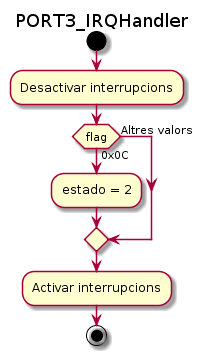
\includegraphics[scale=.6]{PORT3_IRQHandler}
  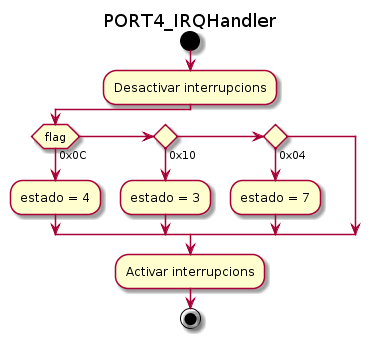
\includegraphics[scale=.6]{PORT4_IRQHandler}
\end{figure}

\begin{figure}[H]
  \centering
  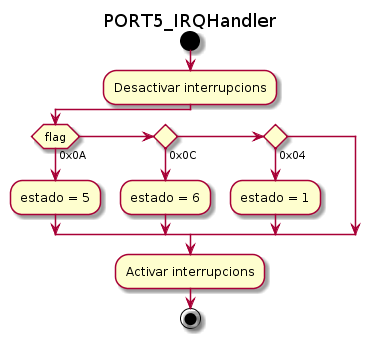
\includegraphics[scale=.6]{PORT5_IRQHandler}
\end{figure}

\begin{figure}[H]
  \centering
  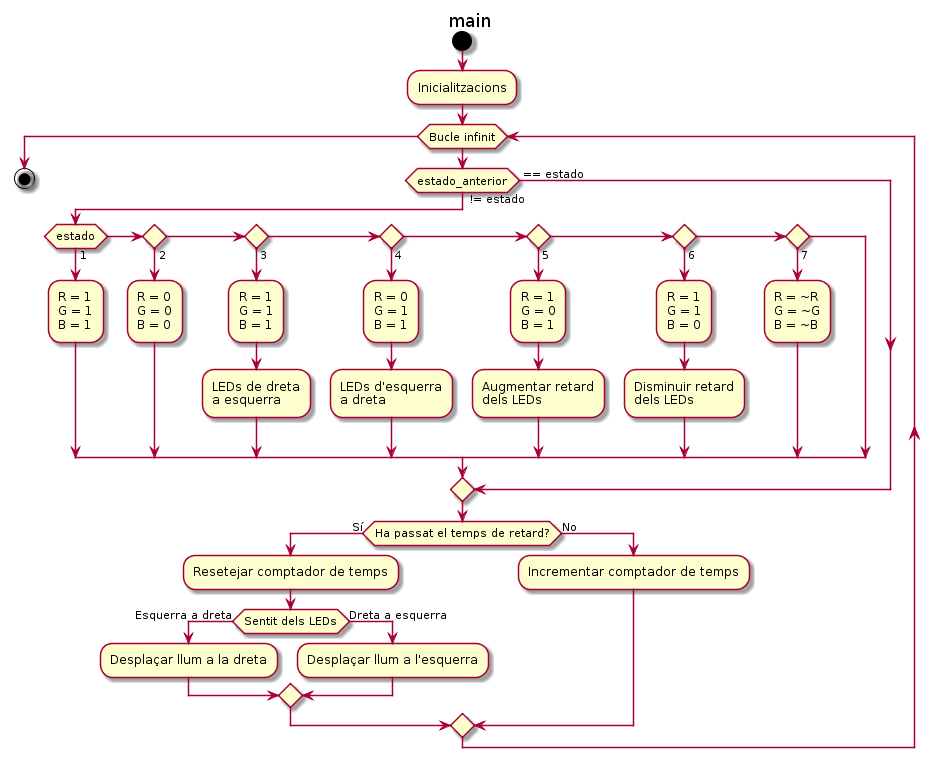
\includegraphics[width=\textwidth]{main}
\end{figure}

\end{document}
